


\documentclass[25pt, a0paper, portrait, margin=20mm]{tikzposter}

 % Commands
\newcommand{\bs}{\textbackslash}   % backslash
\newcommand{\cmd}[1]{{\bf \color{red}#1}}   % highlights command
\tikzposterlatexaffectionproofon

 % Title, Author, Institute
\title{We love TikZ Posters}
\author{Pascal Richter \& Dr. Richard Barnard}
\institute{MathCCES, RWTH Aachen University, Germany}

 % Set colortheme
 % (default, anil, armin, edgar, emre, hanna, james, kai, lena, manuel,
 % martin, max, nicolas, pascal, peter, philipp, richard, roman, stefanie,
 % vinay)
\usecolortheme{lena}

 % Change some colors
\definecolor{framecolor}{named}{black}

\settitlebodystyle{rectangular}
\setblocktitlestyle{rounded}
\setblockbodystyle{shaded}

 % Begin document
\begin{document}

  % Title block
\titleblock[left fig=logoL.png, right fig=logoR.png, left fig height=7cm, right fig height=7cm,embedded]

\block[l]{Formatting Options}{
To generate a poster, you can use the \textsf{tikzposter} class with
    the command \\
    \cmd{\bs documentclass[}\emph{options}\cmd{]\{tikzposter\}}. As options you can set some or all of: font size, paper size, orientation, \cmd{margin},\cmd{inner margin},\cmd{title inner sep}, \cmd{title to block block vertical space},\cmd{block title inner sep},\cmd{block body inner sep}, \cmd{blocktitle width ratio}, \cmd{block title max width}, \cmd{block vertical space},\cmd{col space}, and \cmd{subcol space}.  This document was created via\\
\vspace{1em}
\cmd{\bs documentclass[25pt, a0paper, portrait, margin=20mm]\{tikzposter\}}.\\
\vspace{1em}
Additionally, shapes for the different blocks can be altered by changing the styles in the preamble.  This poster uses\\
\vspace*{1em}
 \cmd{\bs settitlebodystyle\{rectangular\}}, (only effects if the title is not embedded) \\
 \cmd{\bs setblocktitlestyle\{rounded\}}, \\
 \cmd{\bs setblockbodystyle\{shaded\}}. \\
}

\begin{columns}

 % Set first column
\column{0.52}

 % First column - first block
\block[l]{Title Blocks}{
    At first, a title should be set.
    \begin{itemize}
    \item Title elements are \cmd{\bs title}, \cmd{\bs author} and
        \cmd{\bs institute.}
    \item The title block is created by \cmd{\bs titleblock}
    \item There are two types of title blocks:
        \begin{itemize}
            \item not embedded block with rounded block edges separated from the edge of the poster,
            \item embedded blocks which cover the whole poster width.
        \end{itemize}
        The default is not embedded. The type can be set via setting \cmd{embedded = <}\emph{true or false}\cmd{>}; alternatively, \cmd{embedded} sets it as true.
    \item Also, the title block may have logos on the right, left, or both.  This is set via \cmd{left fig, left fig height, right fig} and \cmd{right fig height}.
    \item The title matter may be placed below the title block by setting \cmd{separated=<}\emph{true or false}\cmd{>}; alternatively, \cmd{separated} sets it as true.  The default is not separated.
    \end{itemize}
    The title here was generated by \\ \cmd{\bs titleblock[left fig=logoL.png, right fig=logoR.png, left fig height=7cm, right fig height=7cm]}
}
 % First column -second block
 \block[c,width=0.6\colwidth] {Normal Blocks}{
    Standard blocks may be created with the command \\ \cmd{\bs block[}\emph{options}\cmd{]\{}\emph{title}\cmd{\}\{}\emph{text}\cmd{\}}. Where the options are alignment (either \emph{l,c,r}) for the title and block width which can be defined absolutely or relatively. No title is shown when the title is left blank.  This block was generated by \\[1em]
    \cmd{\bs block[c,width=0.9\bs colwidth]\{Normal Blocks\}\{}\emph{CONTENTS}\cmd{\}}\\[1em]
    where the reference to \cmd{\bs colwidth} will be explained in the next block.
}
 % Set second column
\column{0.48}

 % Second column - first block
\block[c]{Columns}{
     The page can be divided for some segment of the poster into columns of vertically aligned blocks by using the environment \cmd{ columns}.  Within this environment, a column is begun with the command, for instance, \\
     \vspace{1em}
     \cmd{\bs column\{}0.40\cmd{\}}\\
     \vspace{1em}
     for a column of blocks center aligned along a vertical line with default width of $40\%$ of the available width.
     Following this, additional blocks are created which will be aligned into this column until a new column is called
     or the environment is ended.  The current column can be used for reference by the variable \cmd{\bs colwidth}.
}

 % Second column - third block
\block{Subblocks}{
    If, inside a column, additional subcolumns should be created, the environment \cmd{subcolumns} may be created.
    Subcolumns are then created by, for instance,\\
     \vspace{1em}
     \cmd{\bs subcolumn\{}0.40\cmd{\}}\\
     \vspace{1em}
     where the relative width is with respect to \cmd{\bs colwidth}.  The current subcolumn's width is stored in \cmd{\bs subcolwidth}.
    }

 % Second column - subblocks
\begin{subcolumns}
    \subcolumn{0.3} \block{}{First subblock.} \block{}{Second subblock}
    \subcolumn{0.5} \block{Images}{You can put images in of course,
        by using \cmd{\bs subcolwidth} as width for the image. Note, the \cmd{figure} environment is unavailable.  However, the caption package can be created to caption images.}
    \subcolumn{0.2} \block{}{\includegraphics[width=\subcolwidth]{logo}}
\end{subcolumns}

\block{Other blocks}{Text}

\end{columns}

\block{Blocks after ending the columns}{Text}

\begin{columns}
\column{0.3}
\block{Making new columns}{ TikZ Picture by Dominique W\"urtz -- Intersecting rings \\
\def\ringa{(-1,0) circle (2) (-1,0) circle (3)}
\def\ringb{(1,0) circle (2) (1,0) circle (3)}
\begin{center}
    \begin{tikzpicture}[scale=1.4]
        \begin{scope}[even odd rule]
            \clip \ringa;
            \fill[fill=orange] \ringb;
        \end{scope}
        \draw \ringa;
        \draw \ringb;
    \end{tikzpicture}
    \end{center}
}
\column{0.4}
\block{Title}{TikZ Picture by Thomas G. Kristensen -- Yin and yang \\
\begin{center}
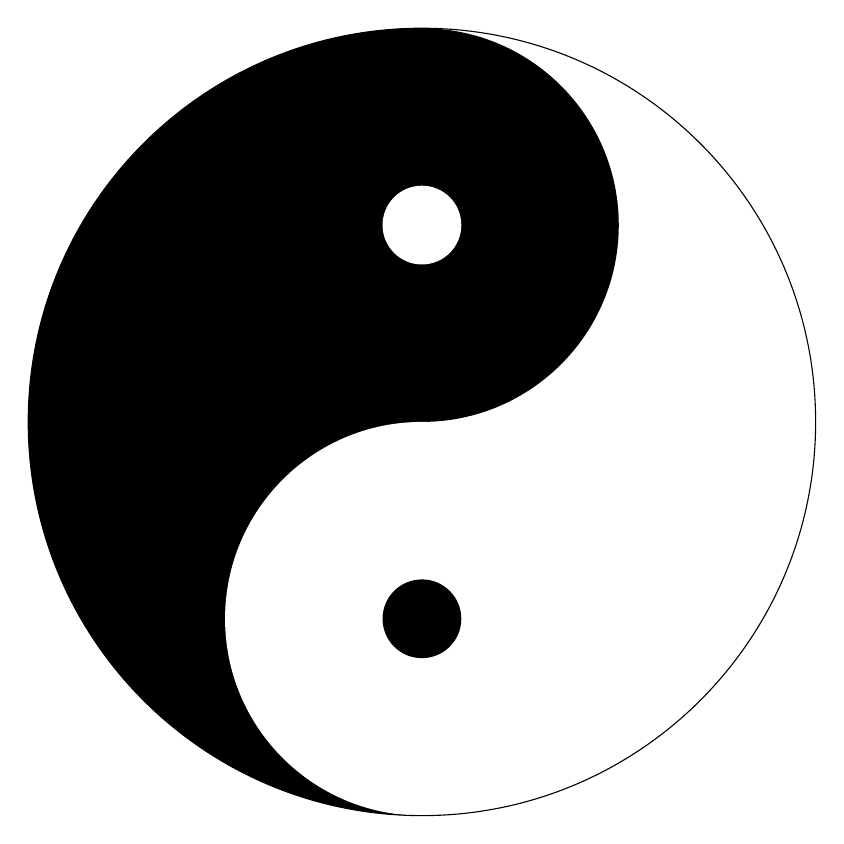
\begin{tikzpicture}[scale=5]
  \begin{scope}
    \clip (0,0) circle (1cm);
    \fill[black] (0cm,1cm) rectangle (-1cm, -1cm);
  \end{scope}
  \fill[black] (0,0.5) circle (0.5cm);
  \fill[white] (0,-0.5) circle (0.5cm);
  \fill[white] (0,0.5) circle (0.1cm);
  \fill[black] (0,-0.5) circle (0.1cm);
  \draw (0,0) circle (1cm);
\end{tikzpicture}
\end{center}
}
\column{0.3}
\block{Title}{TikZ Picture by Paul Gaborit -- The Olympic rings \\
\begin{center}
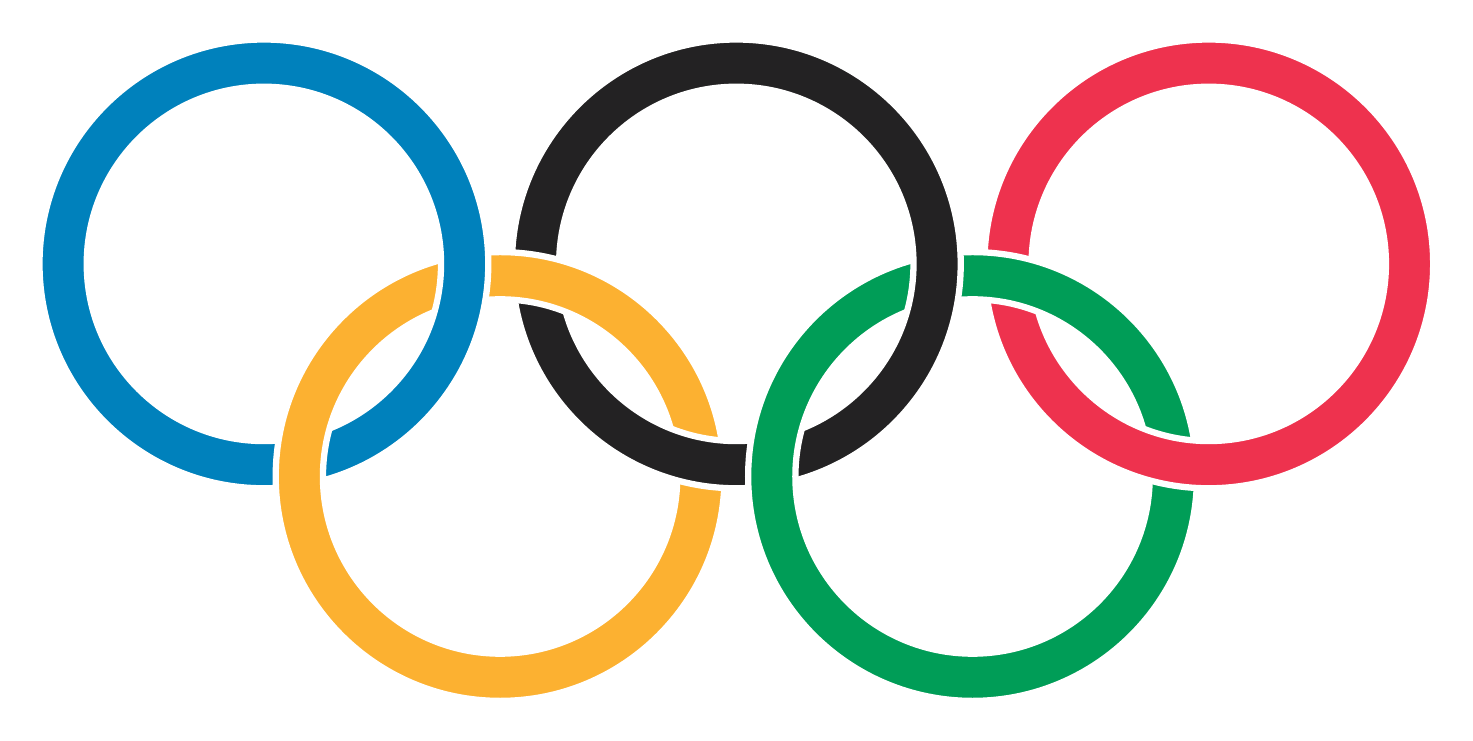
\begin{tikzpicture}[scale=1.5]
 \definecolor{r1}{RGB}{0,129,188}
 \definecolor{r2}{RGB}{252,177,49}
 \definecolor{r3}{RGB}{35,34,35}
 \definecolor{r4}{RGB}{0,157,87}
 \definecolor{r5}{RGB}{238,50,78}
 \begin{scope}
   \clip (-6,2) rectangle (6,-.9);
   \foreach \col/\xp/\yp in {
     r5/4/0, r4/2/-1.8, r3/0/0,
     r2/-2/-1.8, r1/-4/0
   } {
     \path[draw=white,line width=.08cm,
     fill=\col,even odd rule]
     (\xp, \yp) circle (1.9cm)
     (\xp, \yp) circle (1.5cm);
   }
 \end{scope}
 \begin{scope}
   \clip (-6,-.9) rectangle (6,-3.8);
   \foreach \col/\xp/\yp in {
     r1/-4/0, r2/-2/-1.8, r3/0/0,
     r4/2/-1.8, r5/4/0
   } {
     \path[draw=white,line width=.08cm,
     fill=\col,even odd rule]
     (\xp, \yp) circle (1.9cm)
     (\xp, \yp) circle (1.5cm);
   }
 \end{scope}
\end{tikzpicture}
\end{center}
}
\end{columns}
\block{Title}{Text}

\end{document}


